%%%%%%%%%%%%%%%%%%%%%%%%%%%%%%%%%%%%%%%%%
% baposter Portrait Poster
% LaTeX Template
% Version 1.0 (15/5/13)
%
% Created by:
% Brian Amberg (baposter@brian-amberg.de)
%
% This template has been downloaded from:
% http://www.LaTeXTemplates.com
%
% License:
% CC BY-NC-SA 3.0 (http://creativecommons.org/licenses/by-nc-sa/3.0/)
%
%%%%%%%%%%%%%%%%%%%%%%%%%%%%%%%%%%%%%%%%%

%----------------------------------------------------------------------------
%	PACKAGES AND OTHER DOCUMENT CONFIGURATIONS
%----------------------------------------------------------------------------

\documentclass[a0paper,landscape,fontscale=0.395]{baposter}

\usepackage[font=small,labelfont=bf]{caption} % Required for specifying captions to tables and figures
\usepackage{booktabs} % Horizontal rules in tables
\usepackage{enumitem} % To change spacing in itemize and enumerate lists
\usepackage{multicol}
\usepackage{relsize} % Used for making text smaller in some places
\usepackage{amsfonts, amsmath, amsthm, amssymb} % For math fonts, symbols and environments
\usepackage{wrapfig} % Allows wrapping text around tables and figures
\usepackage[export]{adjustbox}% http://ctan.org/pkg/adjustbox
\usepackage{palatino} % Uncomment to use the Palatino font
\usepackage{graphicx} % Required for including images
\usepackage{graphbox}
\usepackage{color}
\usepackage{mathtools}
\usepackage{hyperref}

\graphicspath{{figures/}} % Directory in which figures are stored

\definecolor{bordercol}{RGB}{256,256,256} % Border color of content boxes
\definecolor{headercol1}{RGB}{51,0,111} % Background color for the header in the content boxes (left side)
\definecolor{headercol2}{RGB}{51,0,111} % Background color for the header in the content boxes (middle)
\definecolor{headerfontcol}{RGB}{256,256,256} % Text color for the header text in the content boxes
\definecolor{boxcolor}{RGB}{256,256,256} % Background color for the content in the content boxes

\newenvironment{Figure}
  {\par\medskip\noindent\minipage{\linewidth}}
  {\endminipage\par\medskip}

\DeclarePairedDelimiterX{\norm}[1]{\lVert}{\rVert}{#1}
\DeclareMathOperator{\Tr}{Tr}

\begin{document}

\begin{poster}{
    columns=3,
    grid=false,
    headerheight=0.1\textheight,
    borderColor=bordercol, % Border color of content boxes
    headerColorOne=headercol1, % Background color for the header in the content boxes (left side)
    headerColorTwo=headercol2, % Background color for the header in the content boxes (middle)
    headerFontColor=headerfontcol, % Text color for the header text in the content boxes
    boxColorOne=boxcolor, % Background color for the content in the content boxes
    headershape=roundedright, % Specify the rounded corner in the content box headers
    headerfont=\Large\sf\bf, % Font modifiers for the text in the content box headers
    textborder=rectangle,
    background=none,
    headerborder=open, % Change to closed for a line under the content box headers
    boxshade=plain
}
{}
%
%----------------------------------------------------------------------------
%	TITLE AND AUTHOR NAME
%----------------------------------------------------------------------------
%
{\sf\bf Deep learning for analysis of diffusion-MRI based white matter tractometry} % Poster title
{%
    \vspace{1em}
    Joanna Qiao{$^1$}, Jason Yeatman{$^2$}, Ariel Rokem{$^1$}, Adam Richie-Halford{$^2$}
    \\ Contact: arokem@uw.edu, adamrh@stanford.edu \hspace{0.5em} \null \\ % Author names (cont)
    {\smaller%
        1. University of Washington, %
        2. Stanford University %
        \hfill %
    }
} % Author affiliations and email addresses
{%

\includegraphics[align=c,height=3.00cm]{logos/UWlogo.png}%

\includegraphics[align=c,height=3.20cm]{logos/stanford_logo.png}%
} % University/lab logos
\vspace{-10em}

%----------------------------------------------------------------------------
%	INTRODUCTION
%----------------------------------------------------------------------------

\headerbox{Introduction}{name=introduction, column=0, row=0}{

\begin{itemize}[nosep, leftmargin=*]
    \item Tractometry uses diffusion MRI (dMRI) to quantify brain tissue properties within white matter connections \emph{in vivo} \cite{yeatman2012}.
    \item The Healthy Brain Network Processed Open Derivatives is a large (n>2,000) datset of dMRI that has been processed and automatically QC'd\cite{RichieHalfordCieslak2022HBNPOD2, alexander2017hbn}.
    \item The pyAFQ software was used to create tract profiles for statistical analysis \cite{Kruper2021evaluating}.
    \item In previous work, we demonstrated that regularized regression provides accurate predictions of individual age in HBN from tractometry data (WM-based ``brain age'')\cite{richford2021sgl}.
\end{itemize}

\vspace{0.5em}
\noindent\textbf{%
    \underline{Question}: %
    Would convolutional neural networks provide improvements in inferences from tractometry?%
}
\vspace{0.5em}}

\headerbox{Methods}{name=methods, column=0, below=introduction}{
\begin{itemize}[nosep, leftmargin=*]
\end{itemize}


\begin{minipage}[b]{1\linewidth}
    \large
    \begin{minipage}[b]{0.33\linewidth}
    \textbf{A}\\
    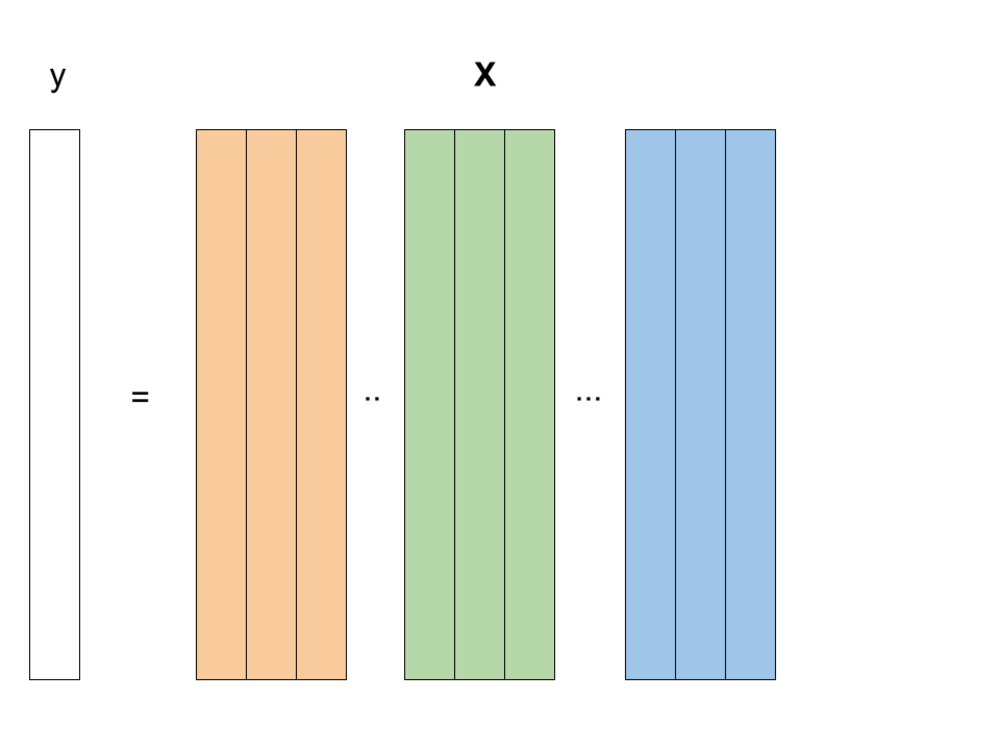
\includegraphics[height=4.5cm]{figures/linear-model.pdf}
    \end{minipage}
    \hspace{0.25cm}
    \begin{minipage}[b]{0.33\linewidth}
    \textbf{B}\\
    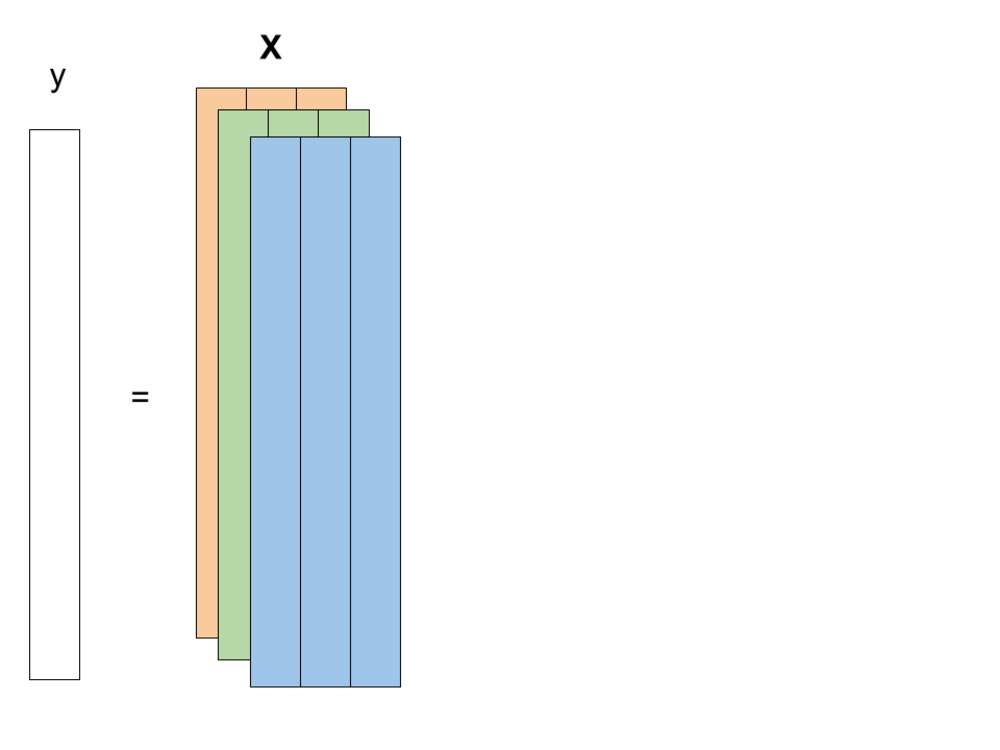
\includegraphics[height=4.5cm]{figures/linear-to-convnet.pdf}
    \end{minipage}
    \begin{minipage}[b]{0.33\linewidth}
    \textbf{C}\\
    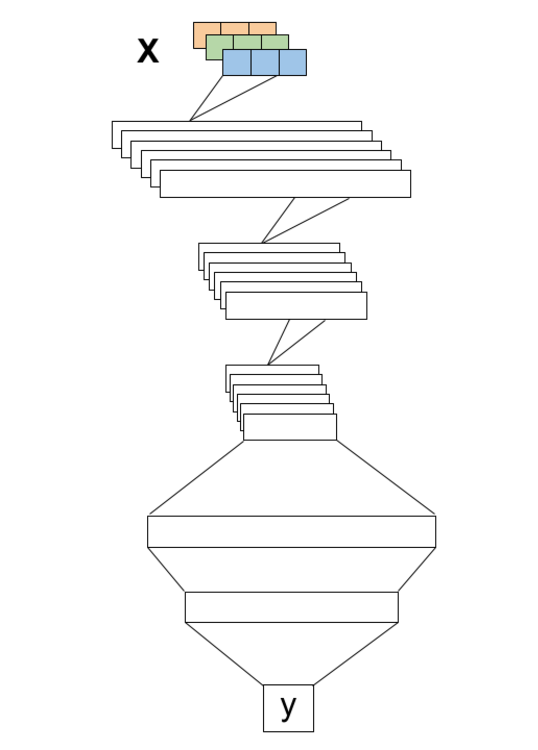
\includegraphics[height=4.5cm]{figures/convnet-schematic.pdf}
    \end{minipage}
 \end{minipage}

In a linear tractometry model, $\textbf{y} = \beta X$ (\textbf{A}), to move towards a convolutional neural networks, we stack the data from different tracts and metrics (FA, MD, MK) as different measurement ``channels'' (\textbf{B}). Training samples are then passed to a network (\textbf{C}).
}

%----------------------------------------------------------------------------
%	CONCLUSION
%----------------------------------------------------------------------------

\headerbox{Conclusion and future work}{name=conclusion, column=0, below=methods}{

\begin{itemize}[nosep, leftmargin=*]
    \item We present a large preprocessed dMRI dataset for the study of pediatric
    mental health and structural brain connectivity.

    \begin{itemize}[nosep, leftmargin=*]
        \item 2,136 subjects, aged 5-21
        \item preprocessed DWI
        \item including QC ratings created from a combination of expert ratings and citizen scientists
        \item openly available on FCP-INDI
    \end{itemize}

    \item HBN-POD2 is amenable to different dMRI analysis, including tractometry, graph theoretical analysis, and combinations with fMRI.

    \item Future work:
    \begin{itemize}[nosep, leftmargin=*]
        \item HBN-POD2 will grow as HBN reaches its 10,000 participant goal.
        \item Develop a deep learning model for QC of future releases
        without the need for citizen science ratings.
    \end{itemize}
\end{itemize}

}

%----------------------------------------------------------------------------
%	RESULTS 1
%----------------------------------------------------------------------------

\headerbox{Results Control}{name=qc, column=1, span=2, row=0}{

\begin{itemize}[noitemsep, leftmargin=*]
    \item Six dMRI experts rated 200 participants’ processed data on a 1-5 scale using the dmriprep-viewer interface \url{https://www.nipreps.org/dmriprep-viewer})
    \item We found excellent inter-rater reliability: ICC3k=0.93 (95\% CI: [0.91, 0.94]) Ratings are available in \url{https://github.com/richford/hbn-pod2-expert-qc}.
    \item We call this subset the ``gold standard'' QC dataset.
    \item But the size of HBN-POD2 makes expert QC on the full dataset prohibitive, we estimate QC of the full dataset would take each FTE expert rater ~200 hours.
\end{itemize}

\vspace{0.5em}
\noindent\textbf{%
    \underline{Challenge}: %
    Generate QC labels for a large dMRI dataset when expert ratings are prohibitively time consuming.%
}
\vspace{0.5em}

\begin{itemize}[noitemsep, leftmargin=*]
    \item Based on the SwipesForScience framework
    (https://swipesforscience.org/; \cite{keshavan2019citizen}), we created a
    citizen science web-app that presents static/dynamic views of b=0 maps and
    directionally-encoded FA maps for a binary (pass/fail) decision for 1,653
    HBN subjects.
    \item 374 citizen scientists provided $587,778$ ratings (of these, 133
    citizen scientists provided $>3,000$ votes each) for a mean of $>50$ ratings
    per slice (or $>200$ ratings per subject).
    \item We then trained a gradient boosting model (XGB) to predict expert scores
    based on a combination of citizen science ratings and automated QSIPrep QC
    metrics, attaining $R^2 = 0.80$ on a held-out test set from the ``gold standard.''
    \item A separate model trained on only the QSIPrep QC metrics attained $R^2 = 0.68$,
    demonstrating the added value of the citizen science raters.
\end{itemize}

\begin{multicols}{3}
    \begin{Figure}
        \centering
        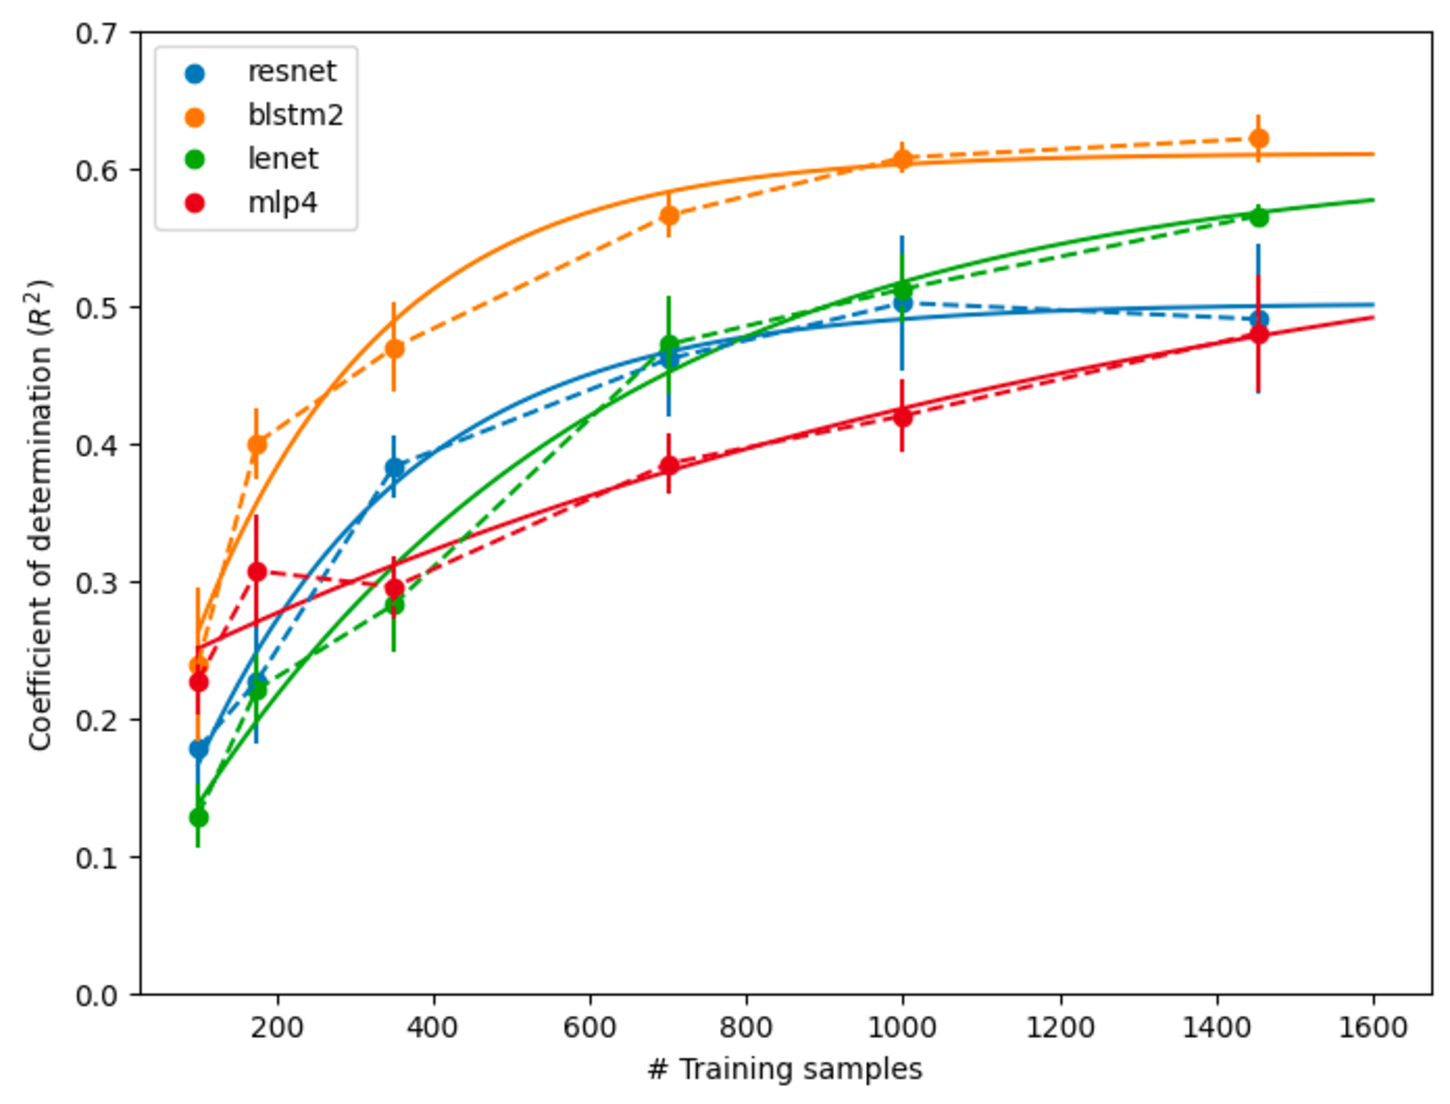
\includegraphics[width=0.33\linewidth]{figures/results_no_aug}
        \captionof{figure}{
            {\bf HBN-POD2 quality control (QC) instruments}:
            {\bf (A)} The user interface for citizen science QC. After a
            tutorial, users are asked to give binary pass/fail ratings to
            each subject's color scale fractional anisotropy image. The
            intuitive swipe or click interface allows citizen scientists to
            review more images than is practical for expert review. Expert
            reviewers use the more advanced qsiprep-viewer interface, where
            they can
            {\bf (B)} view the distribution of QC metrics for the entire
            study using interactive scatterplots and violin plots, and
            {\bf (C)} inspect Individual subjects' preprocessing results,
            including corrected dMRI images, frame displacement, q-space
            sampling distributions, registration information, and a DTI
            model.
        }
    \end{Figure}
    \columnbreak
    \begin{Figure}
        \centering
        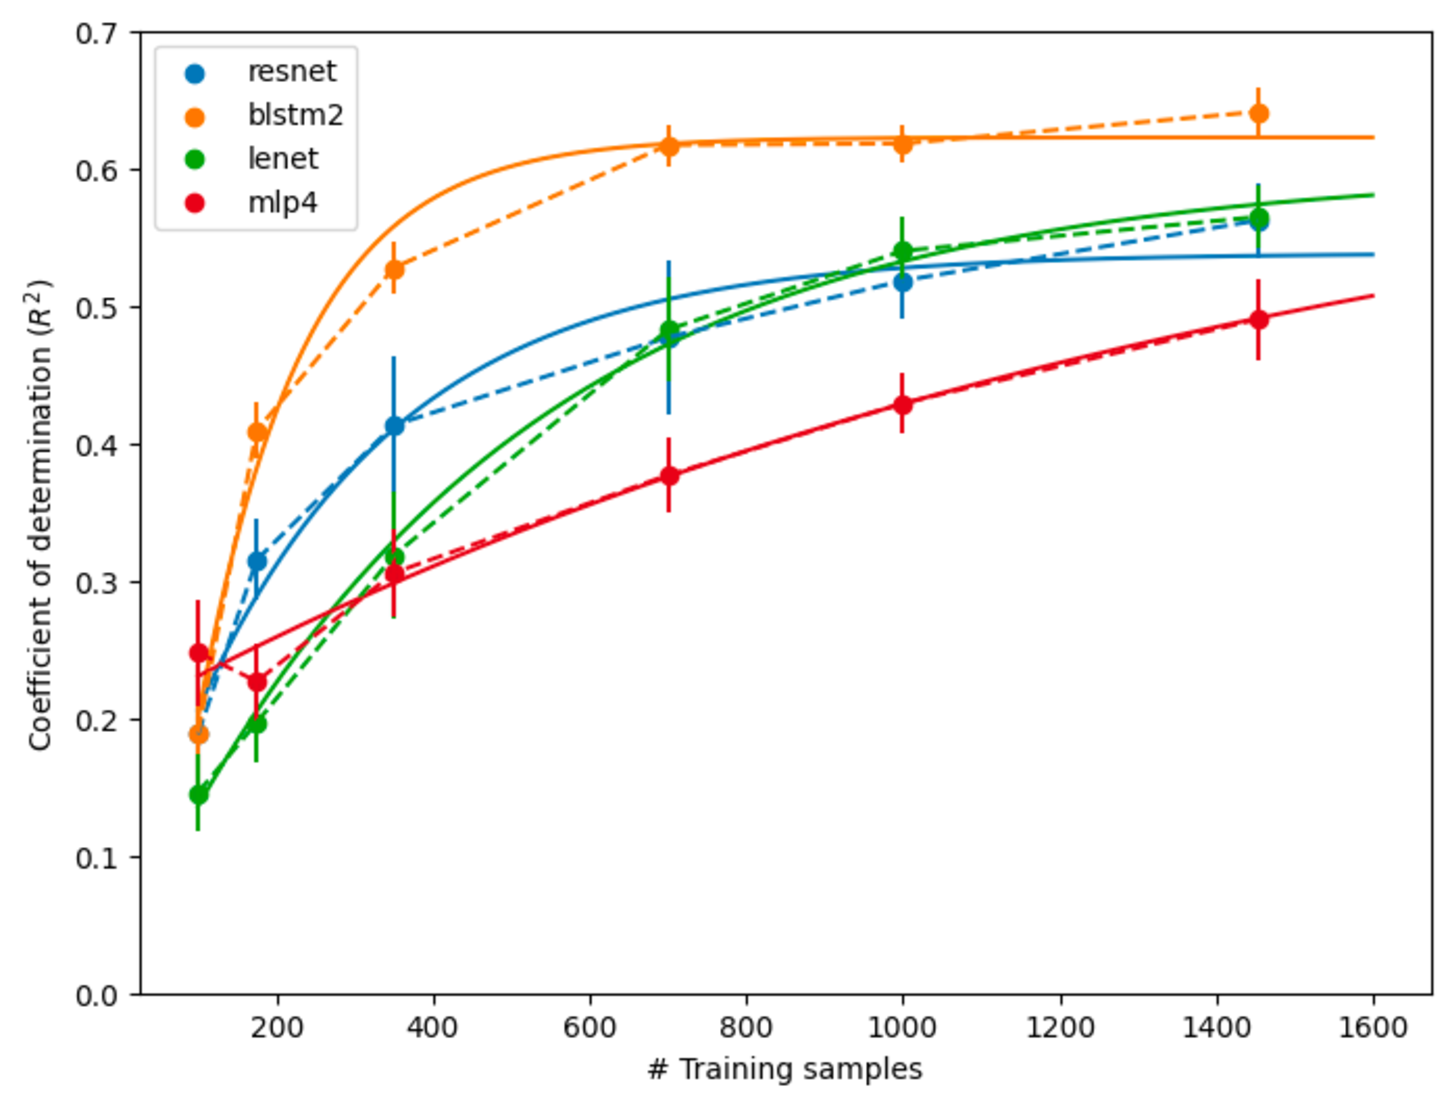
\includegraphics[width=0.33\linewidth]{figures/results_low_aug.pdf}
        \captionof{figure}{
            {\bf HBN-POD2 quality control (QC) results}:
            Six dMRI experts (with anonymized names) rated a subset of
            200 subjects, with acceptable inter-rater reliability:
            $\textbf{ICC3k} = 0.930 (95\% CI: [0.91, 0.94])$,
            $\textbf{ICC3} = 0.688 (95\% CI: [0.64, 0.74])$,
            $\langle \kappa \rangle = 0.648$.
            We trained a gradient boosting model (XGB) on the average expert
            rating, obtaining $R^2 = 0.80$ on a held-out test set.  Treating XGB
            as a seventh expert rater, preserves inter-rater reliability:
            $\textbf{ICC3k} = 0.945 (95\% CI: [0.93, 0.96])$,
            $\textbf{ICC3} = 0.709 (95\% CI: [0.66, 0.75])$.
            This entitles us to extend it's ratings to the entire HBN-POD2
            dataset.
        }
    \end{Figure}

    \columnbreak
    \begin{Figure}
        \centering
        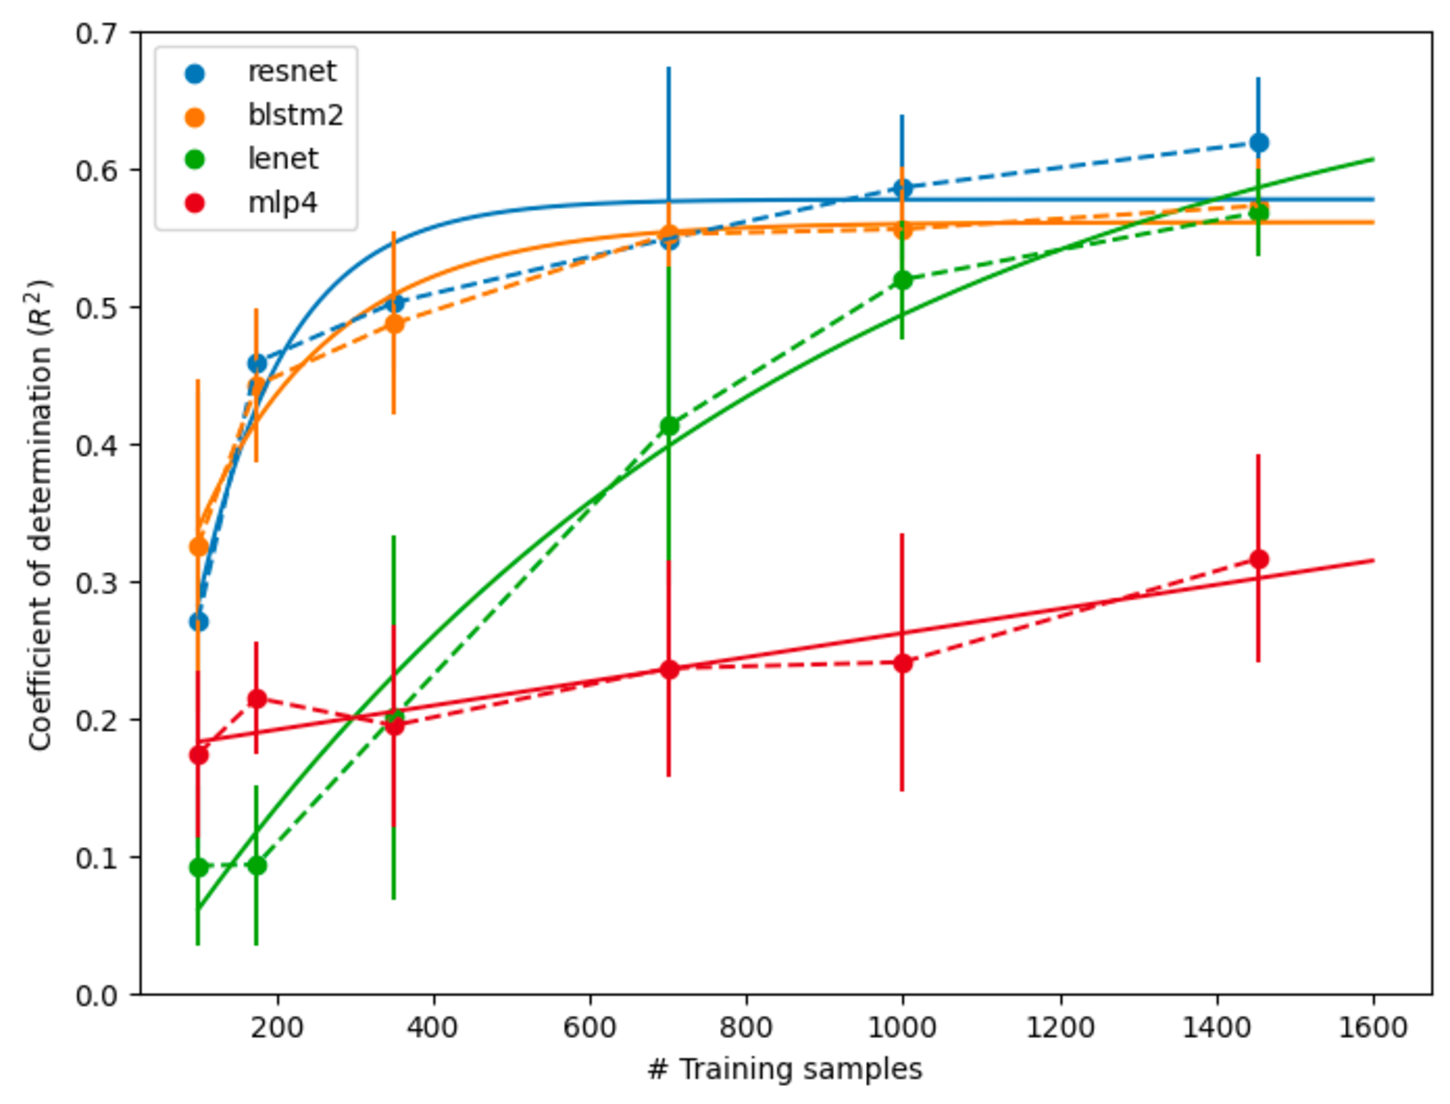
\includegraphics[width=0.33\linewidth]{figures/results_high_aug.pdf}
        \captionof{figure}{
            {\bf HBN-POD2 quality control (QC) results}:
            Six dMRI experts (with anonymized names) rated a subset of
            200 subjects, with acceptable inter-rater reliability:
            $\textbf{ICC3k} = 0.930 (95\% CI: [0.91, 0.94])$,
            $\textbf{ICC3} = 0.688 (95\% CI: [0.64, 0.74])$,
            $\langle \kappa \rangle = 0.648$.
            We trained a gradient boosting model (XGB) on the average expert
            rating, obtaining $R^2 = 0.80$ on a held-out test set.  Treating XGB
            as a seventh expert rater, preserves inter-rater reliability:
            $\textbf{ICC3k} = 0.945 (95\% CI: [0.93, 0.96])$,
            $\textbf{ICC3} = 0.709 (95\% CI: [0.66, 0.75])$.
            This entitles us to extend it's ratings to the entire HBN-POD2
            dataset.
        }
    \end{Figure}

    \vspace{2em}
    {\smaller %
        \textsuperscript{\textasteriskcentered} \textbf{ICC3} and \textbf{ICC3k}
        are appropriate when a fixed set of $k$ raters rate each subject (i.e. a
        fully crossed design).  When all subjects are coded by multiple raters
        and the average of their ratings is used for hypothesis testing,
        \textbf{ICC3k} is appropriate.  When a subset of subjects is coded by
        multiple raters and the reliability of their ratings is meant to
        generalize to other subjects rated by only one coder, the single-measure
        \textbf{ICC3} must be used.
    }
\end{multicols}

\begin{itemize}[noitemsep, leftmargin=*]
    \item Treating the new XGB model as an additional expert rater, we attain
    $\textbf{ICC3k} = 0.945 (95\% CI: [0.93, 0.96])$ and
    $\textbf{ICC3} = 0.709 (95\% CI: [0.66, 0.75])$.
    \item The reliability of the XGB model entitles us to apply the XGB ratings
    to the remaining HBN-POD2 scans, generating QC labels for the entire
    dataset.
    \item HBN-POD2 offers open QC metrics, eliminating the need for
    investigators to repeat quality assessment for over 2,000 scans.
\end{itemize}
}

%----------------------------------------------------------------------------
%   REFERENCES
%----------------------------------------------------------------------------

\headerbox{References}{name=references,column=0,span=2,below=conclusion,above=bottom}{

\begin{multicols}{2}
\smaller \smaller % Reduce the font size in this block
\renewcommand{\section}[2]{\vskip 0.05em} % Get rid of the default "References" section title
\nocite{*} % Insert publications even if they are not cited in the poster

% \printbibliography
\bibliographystyle{unsrt}
\bibliography{poster}
\end{multicols}
}

%----------------------------------------------------------------------------
%	ACKNOWLEDGMENTS
%----------------------------------------------------------------------------

\headerbox{Acknowledgments}{name=acknowledgments, column=2, below=conclusion,above=bottom}{

\begin{multicols}{2}
\smaller % Reduce the font size in this block

\includegraphics[height=1.0cm]{logos/nimh-logo.png}


\includegraphics[height=0.75cm]{logos/eSciencelogo.png}

\end{multicols}
}

\end{poster}

\end{document}
